\documentclass{beamer}
\usetheme{Madrid}

\usepackage[utf8]{inputenc}
\usepackage{amsfonts}
\usepackage{amsmath}
\usepackage{amssymb}
\usepackage{mathrsfs}
\usepackage[french]{babel}

%\usepackage{arev}

\usepackage[babel=true]{csquotes}

\usepackage{listings}

\usepackage[center]{caption}
\usepackage{tabularx}


\usepackage{tikz}
\usetikzlibrary{calc, trees, positioning, arrows, shapes, shapes.multipart, shadows, matrix, decorations.pathreplacing, decorations.pathmorphing}

\lstset{escapeinside={<@}{@>}}


\title{Introduction à OpenGL avec GLUT}
%\author[Stott, Bouchiba]{Nikolas Stott \inst{1} \and Hassan Bouchiba \inst{2}}
%\institute[INRIA, MINES]{\inst{1} INRIA Saclay \and \inst{2} MINES ParisTech}
\author[Nikolas Stott]{Nikolas Stott}
\institute[INRIA - CMAP]{INRIA Saclay - CMAP, \'Ecole Polytechnique, Universit\'e Paris-Saclay}
\titlegraphic{
\includegraphics[width=0.3\textwidth]{img/opengl}}
\date{\today}

\AtBeginSection[]
{
\begin{frame}<beamer>{Plan}
\tableofcontents[currentsection]
\end{frame}
}

\newif\iffull
%\fulltrue

\begin{document}

\begin{frame}
\titlepage
\end{frame}

\begin{frame}{Plan}
\tableofcontents
\end{frame}


\section{OpenGL et GLUT : présentation}

\subsection{OpenGL : quoi et comment ?}
\begin{frame}{Qu'est ce qu'OpenGL ?}
	\begin{block}{}
		OpenGL (Open Graphics Library) est une bibliothèque graphique 2D/3D pour des applications 3D (interactives) :
		\begin{itemize}
			\item Interface logicielle bas niveau avec le hardware graphique
			\item 150 commandes différentes pour spécifier objets et opérations
		\end{itemize}
	\end{block}
	\pause
	\begin{block}{}
		OpenGL est indépendant du hardware et utilisé dans différents langages à travers différentes bibliothèques :
		\begin{itemize}
			\item GLU/GLUT en C/C++
			\item Java OpenGL (JOGL) en Java
			\item WEBGL en Javascript
		\end{itemize}
	\end{block}
	\pause
	\begin{block}{}
		OpenGL ne gère pas le fenêtrage ou l'interface graphique.
	\end{block}
\end{frame}


\subsection{GLUT : quoi et comment ?}
\begin{frame}[fragile]
\frametitle{Qu'est ce que GLUT ?}
	\begin{block}{}
		GLUT (OpenGL Utility Toolkit) est une interface de programmation pour OpenGL qui gère le fenêtrage.\\
		GLUT est simple, petit et utile pour apprendre à découvrir OpenGL.
	\end{block}
	\begin{block}{}
		GLUT contient les fonctionnalités suivantes :
		\begin{itemize}
			\item gestion de l'affichage de fenêtres de rendu OpenGL
			\item gestion du temps, d'événements et d'interaction utilisateur
			\item création rapide d'objets primitifs (cube, tétraèdre, sphère, cône, etc) pleins ou maillage seul.
		\end{itemize}
	\end{block}
	\begin{overlayarea}{\textwidth}{5cm}
		\only<1>{
			\begin{columns}[T]
				\begin{column}{0.25\textwidth}
					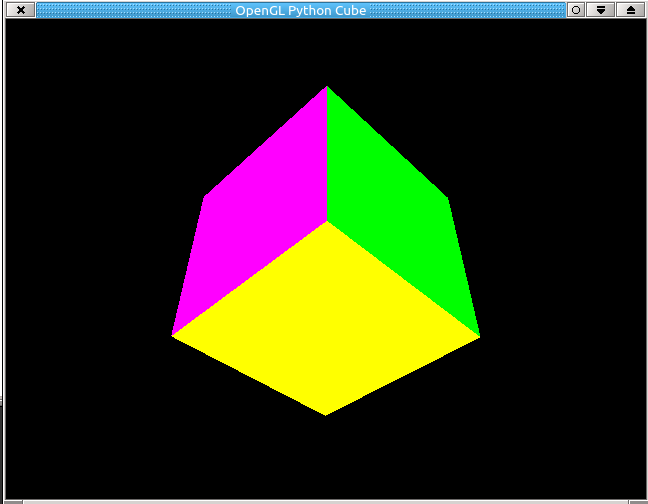
\includegraphics[width=\textwidth]{img/cube}
				\end{column}
				\begin{column}{0.25\textwidth}
					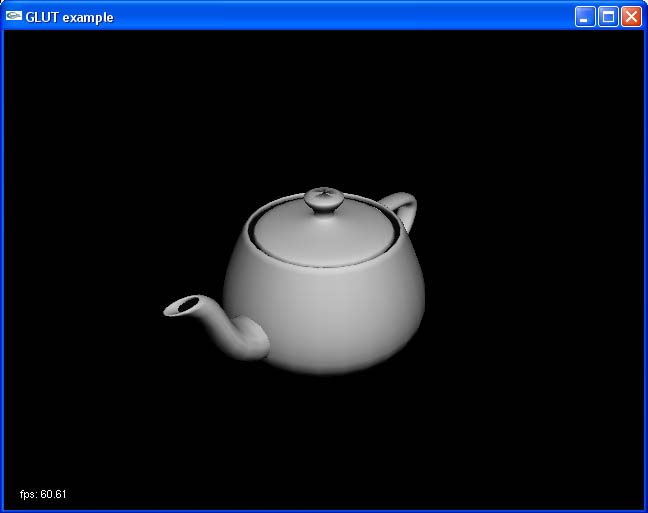
\includegraphics[width=\textwidth]{img/teapot}
				\end{column}
			\end{columns}
		}
		\only<2>{
			\begin{block}{Pour aller plus loin : solutions plus haut niveau}
				\begin{itemize}
					\item Open Inventor (commercial : C++, .NET, Java)
					\item OpenSceneGraph (open source)
				\end{itemize}
			\end{block}
		}
	\end{overlayarea}	
\end{frame}

\begin{frame}{Qu'est ce qu'OpenGL sait faire ?}
	\begin{columns}
		\begin{column}{0.55\textwidth}
			\begin{block}{Modélisation/Visualisation}
				\begin{itemize}
					\item Création de géométries complexes
					\item Habillage de la géométrie : couleur, texture, éclairage...
					\item Visualisation des objets
				\end{itemize}
			\end{block}
		\end{column}
		\begin{column}{0.4\textwidth}
			\centering
			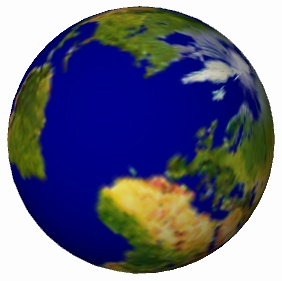
\includegraphics[width=0.8\textwidth]{img/model_earth}
		\end{column}
	\end{columns}
	~\\
	\pause
	\begin{columns}
		\begin{column}{0.4\textwidth}
			\centering
			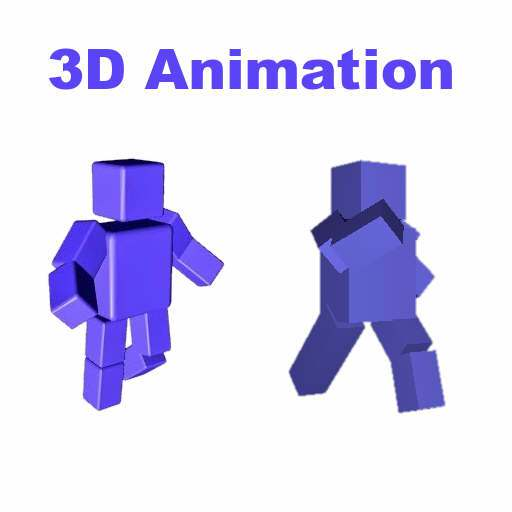
\includegraphics[width=0.8\textwidth]{img/animation}
		\end{column}
		\begin{column}{0.55\textwidth}
			\begin{block}{Animation}
				OpenGL permet d'animer :
				\begin{itemize}
					\item la caméra dans la scène
					\item les objets dans la scène
					\item le maillage des objets
				\end{itemize}
			\end{block}
		\end{column}
	\end{columns}
\end{frame}


%\iffalse

\section{\'El\'ements de modélisation avec OpenGL}

\begin{frame}{La brique de base : le sommet}
	\begin{alertblock}{Dans le cadre de ce cours, ...}
		... l'ordinateur ne conna\^it que le point (vecteur ou \emph{vertex}) !
	\end{alertblock}
	\begin{itemize}
		\item[$\Rightarrow$] Pas de courbe, pas de boule, pas de géométrie lisse.
	\end{itemize}
	\pause
	\begin{block}{Assemblage de géométrie}
		On peut créer des objets simples à partir de sommets:
		\begin{itemize}
			\item lignes (ou \emph{edges}),
			\item polygones (ou \emph{faces}).
		\end{itemize}
	\end{block}
	\begin{itemize}
		\item[$\Rightarrow$] On va assembler ces objets simples en objets plus complexes...
	\end{itemize}
\end{frame}

\begin{frame}{Illustration}
	\begin{figure}
		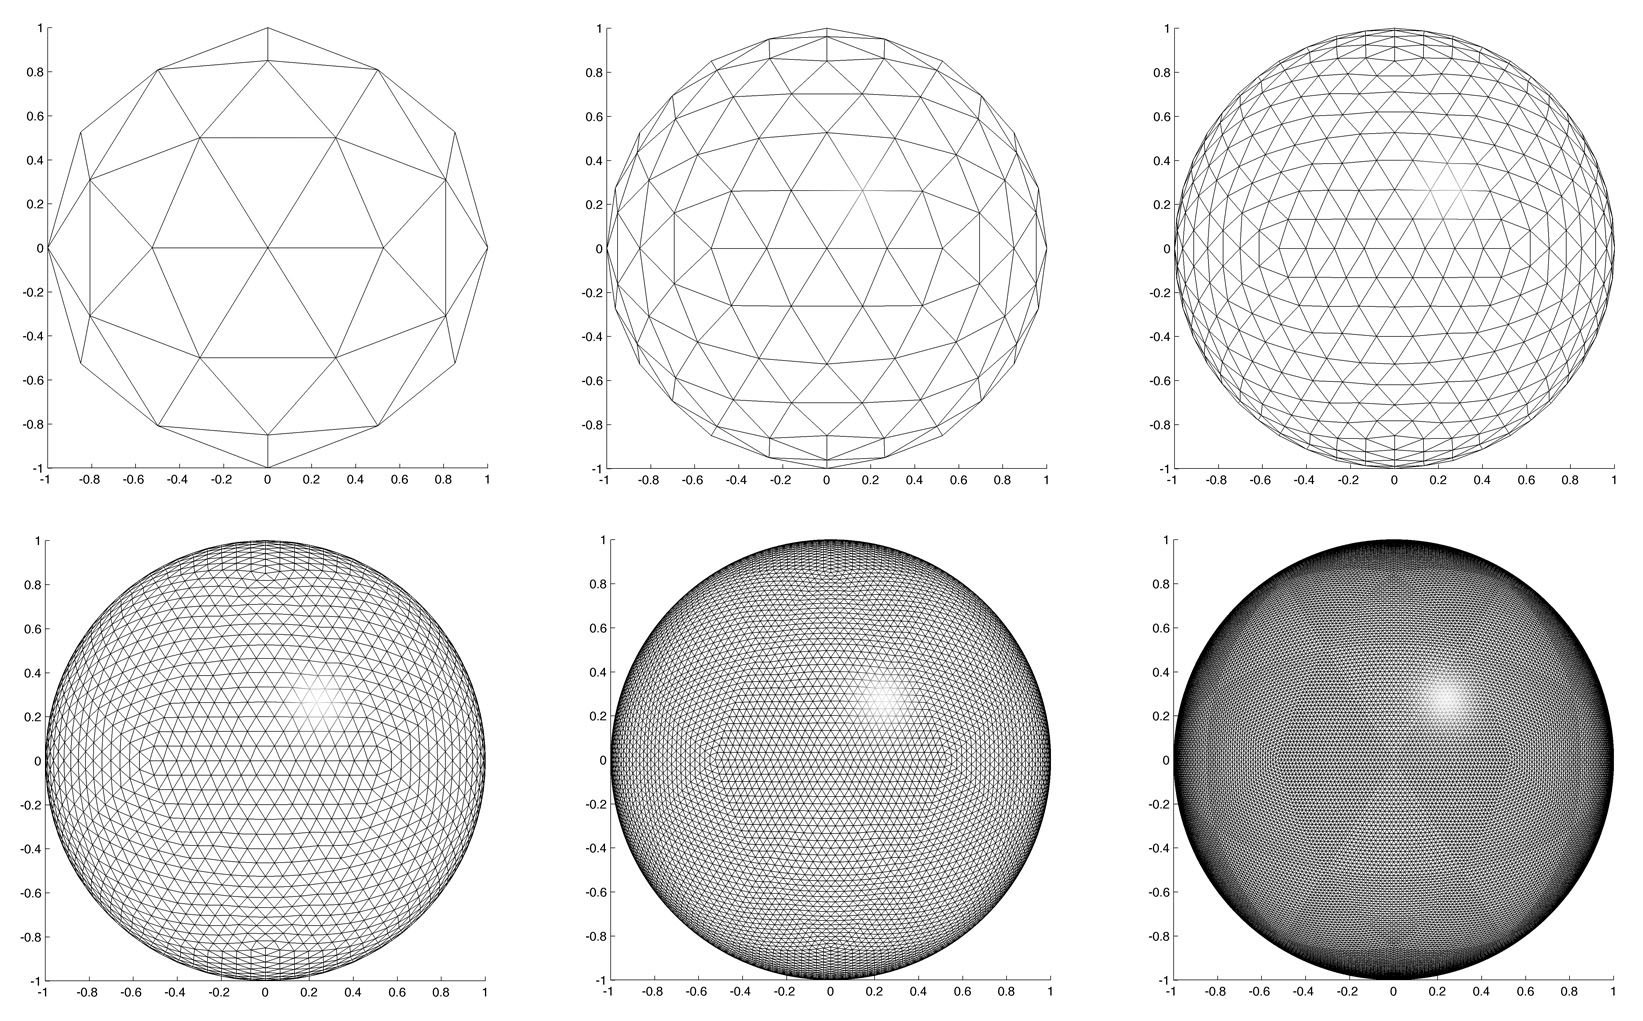
\includegraphics[width=\textwidth]{img/sphere}
	\end{figure}
\end{frame}

\begin{frame}{C'est tout ?}
	\begin{block}{Ce n'est pas suffisant !}
		Il faut également déclarer des informations supplémentaires sur l'objet:
		\begin{columns}
			\begin{column}{0.5\textwidth}
				\begin{itemize}
					\item Orientation des faces,
					\item Couleur des faces,
				\end{itemize}
			\end{column}
			\begin{column}{0.5\textwidth}
				\begin{itemize}
					\item Matériaux de l'objet,
					\item Texture des faces...
				\end{itemize}			
			\end{column}
		\end{columns}
		~\\
		pour qu'il interagisse avec son environnement: lumières...
	\end{block}
	\begin{columns}
		\begin{column}{0.5\textwidth}
			\centering
			\begin{figure}
				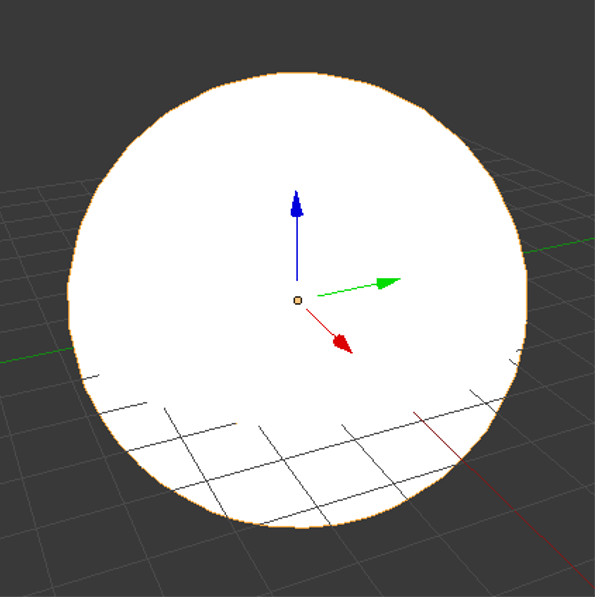
\includegraphics[width=0.6\textwidth]{img/no_shade_sphere}
				\caption*{Sans aucune information:}
			\end{figure}
		\end{column}
		\begin{column}{0.5\textwidth}
			\centering
			\begin{figure}
				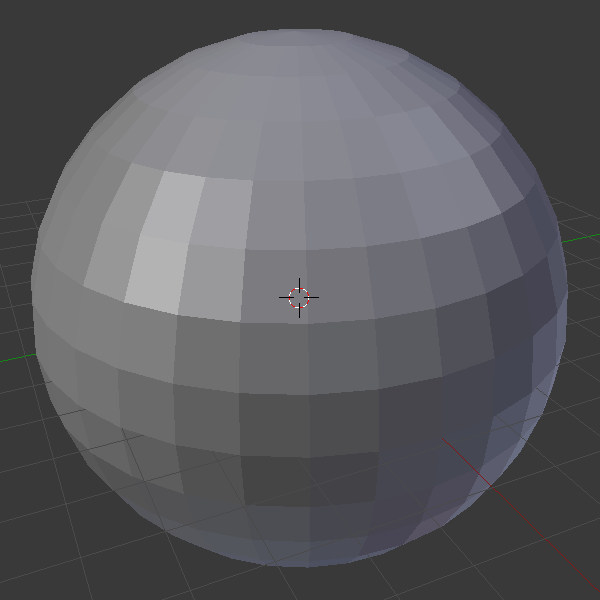
\includegraphics[width=0.6\textwidth]{img/shaded_sphere}
				\caption*{Avec orientation et matériaux:}
			\end{figure}
		\end{column}
	\end{columns}
\end{frame}

\begin{frame}{Pas votre lampe habituelle}
	\begin{block}{Les composantes lumineuses du modèle de Phong}
		Une lumière OpenGL est caractérisée par 5 paramètres:
		\begin{itemize}
			\item Position : vecteur XYZ(W)
			\item Direction du spot : vecteur direction XYZ
			\item Intensité Diffuse : vecteur RGBA
			\item Intensité Spéculaire : vecteur RGBA
			\item Intensité Ambiante : vecteur RGBA
		\end{itemize}
	\end{block}
	\begin{figure}
		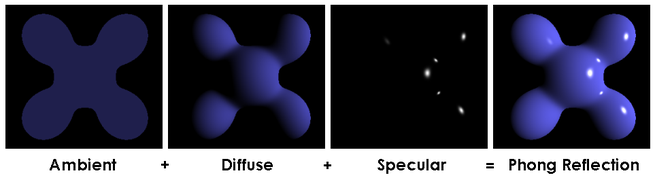
\includegraphics[width=\textwidth]{img/phong}
	\end{figure}
\end{frame}

\begin{frame}{Lumières et Normales}
	\begin{block}{Influence de la normale}
		Sur une face, l'éclairage est calculé avec:
		$
		\left\{
		\begin{tabular}{p{4cm}}
		\text{le vecteur lumineux incident,} \\
		\text{la normale \`a la face}		
		\end{tabular}
		\right.$.
	\end{block}
	\vspace{2mm}
	\begin{columns}
		\begin{column}{0.5\textwidth}
			\centering
			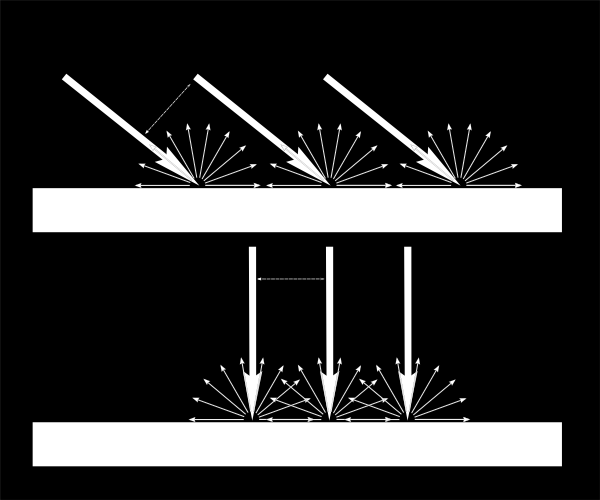
\includegraphics[width=0.8\textwidth]{img/diffuseAngle}
		\end{column}
		\begin{column}{0.5\textwidth}
			\centering
			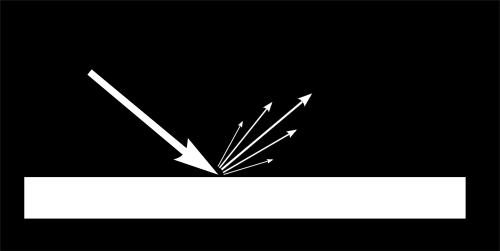
\includegraphics[width=\textwidth]{img/specular}
		\end{column}
	\end{columns}
	\begin{alertblock}{}
		Il faut donner les normales à l'ordinateur: il ne sait pas les calculer...
	\end{alertblock}
\end{frame}

\begin{frame}{Couleur et Textures}
	\begin{columns}
		\begin{column}{0.65\textwidth}
			\begin{block}{Colorier la géométrie}
				\begin{itemize}
					\item Ce sont les sommets qui portent l'information de couleur;
					\item Les faces sont coloriées par interpolation.
				\end{itemize}
			\end{block}
		\end{column}
		\begin{column}{0.3\textwidth}
			\centering
			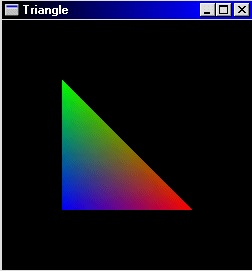
\includegraphics[width=0.6\textwidth]{img/triang}
		\end{column}
	\end{columns}
	\pause
	\begin{block}{Texturer la géométrie}
		\begin{itemize}
			\item On attribue un point de la texture à chaque sommet ;
			\item Les faces sont texturées par interpolation.
		\end{itemize}
	\end{block}
	\begin{columns}
		\begin{column}{0.4\textwidth}
			\centering
			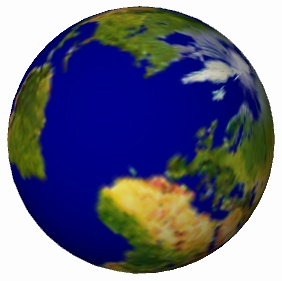
\includegraphics[width=0.7\textwidth]{img/model_earth}
		\end{column}
		\begin{column}{0.6\textwidth}
			\centering
			
\includegraphics[width=1\textwidth]{img/uv_map}
		\end{column}
	\end{columns}
\end{frame}

\begin{frame}{Ce que l'on ne va pas apprendre à faire}
	\begin{alertblock}{Les ombres}
		Les ombres portées ne sont pas calculées automatiquement : c'est à l'utilisateur de les calculer.
	\end{alertblock}
	\begin{alertblock}{Texturer un objet}
		C'est encore à l'utilisateur de définir comment la texture s'applique sur l'objet (UV mapping).
	\end{alertblock}
	\begin{alertblock}{Traitement des shaders}
		Pas de traitement en détail des normales, effets post-traitement, etc... \\
		Pas de canaux de textures améliorés : normal map, bump map, displacement map, ...
	\end{alertblock}
\end{frame}


\section{Les commandes OpenGL}

\subsection{Les commandes basiques}

\begin{frame}
\frametitle{Les briques élémentaires (1)}
	\begin{block}{Les sommets}
		Les sommets sont déclarés par la commande \verb!glVertex3f(x,y,z)!.\\
		Exemples :
		\begin{itemize}
			\item \alert{\verb!glVertex3f(2.4f,4.1f,-0.1f);!}
		\end{itemize}
	\end{block}
%	\begin{columns}
%		\begin{column}{0.7\textwidth}
%			\centering
%			\begin{block}{Par défaut}
%				\begin{itemize}
%					\item \verb!glVertex2?! place les points dans le plan $z = 0$ (et $w = 1$)
%					\item \verb!glVertex3?! fixe $w$ à $1$.
%				\end{itemize}
%			\end{block}
%		\end{column}
%		\begin{column}{0.3\textwidth}
%		\centering
%			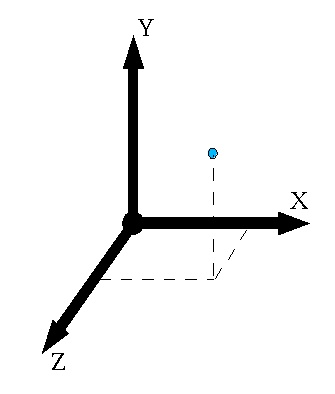
\includegraphics[width=0.7\textwidth]{img/coords}
%		\end{column}
%	\end{columns}
\end{frame}

\begin{frame}[fragile]
\frametitle{Les briques élémentaires (2)}
	\begin{block}{La déclaration de primitive}
		L'assemblage de sommets en faces se fait entre les instructions\\
		\begin{figure}[h]
			\centering
			\begin{tabular}{c}
				\begin{lstlisting}
glBegin(TYPE_DE_LA_PRIMITIVE);
  //declarations optionnelles
  glVertex3f(...);
  ...
  glVertex3f(...);
  //declarations optionnelles
glEnd();
				\end{lstlisting}
			\end{tabular}
		\end{figure}
		Nous verrons les autres déclarations plus loin.
	\end{block}
%	\begin{exampleblock}{}
%		Attention : puisque nous travaillons sur de la géométrie, OpenGL doit être configuré en mode \verb!GL_MODELVIEW! : \verb!glMatrixMode(GL_MODELVIEW);! !
%	\end{exampleblock}
\end{frame}

\begin{frame}
\frametitle{Primitives géométriques disponibles}
\begin{columns}
	\begin{column}{0.3\textwidth}
		\centering		
		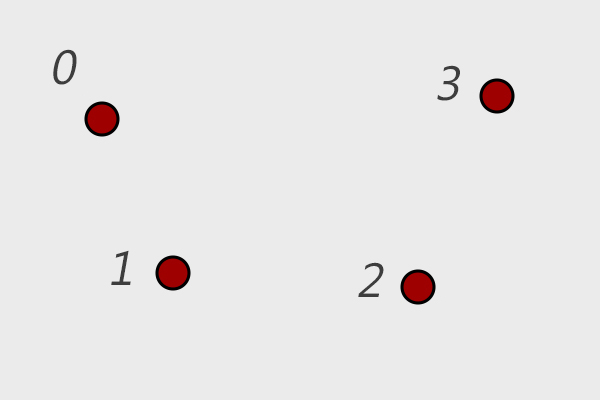
\includegraphics[width=\textwidth]{img/GL_POINTS}
		\\ { GL\_POINTS}
	\end{column}
	\begin{column}{0.3\textwidth}
		\centering	
		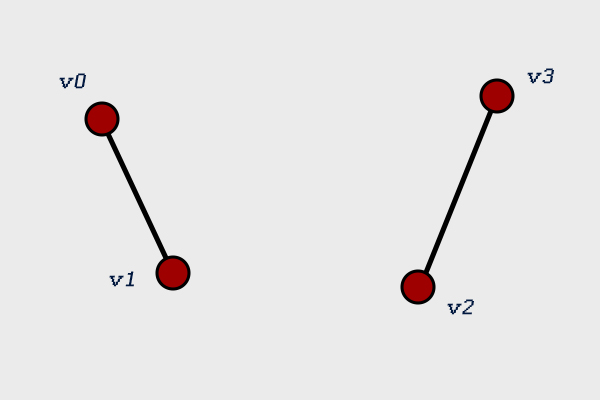
\includegraphics[width=\textwidth]{img/GL_LINES}
		\\ { GL\_LINES}
	\end{column}
%	\begin{column}{0.2\textwidth}
%		\centering	
%		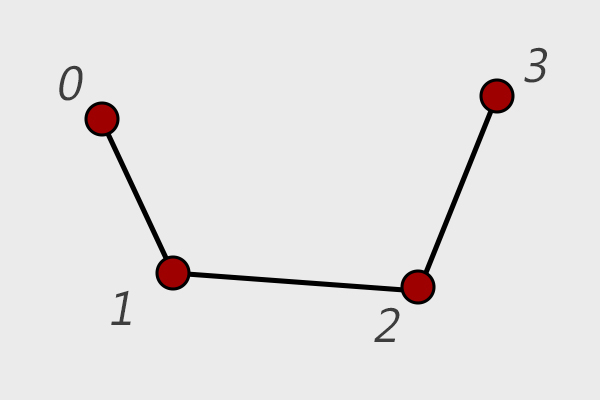
\includegraphics[width=\textwidth]{img/GL_LINE_STRIP}
%		\\ {\tiny GL\_LINE\_STRIP}
%	\end{column}
	\begin{column}{0.3\textwidth}
		\centering	
		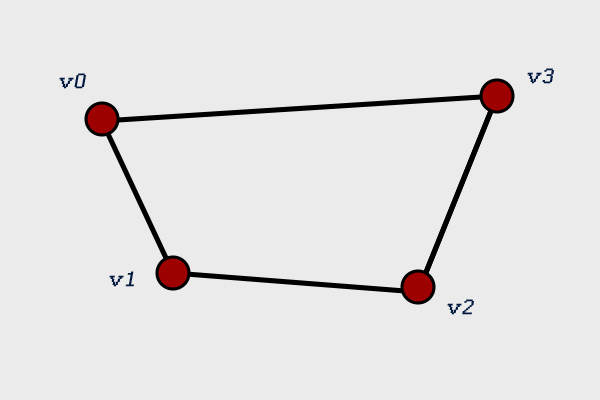
\includegraphics[width=\textwidth]{img/GL_LINE_LOOP}
		\\ { GL\_LINE\_LOOP}
	\end{column}
\end{columns}
~\\
~\\
\pause
\begin{columns}
	\begin{column}{0.3\textwidth}
		\centering		
		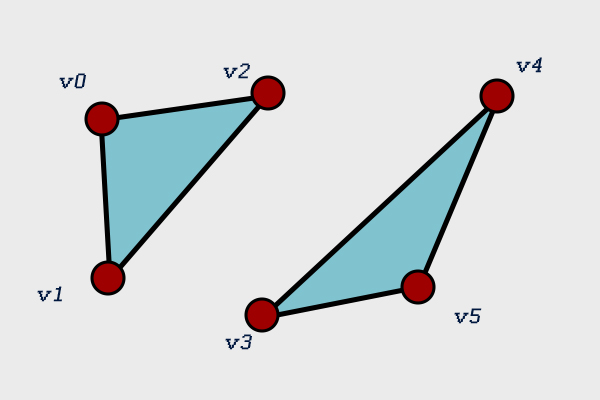
\includegraphics[width=\textwidth]{img/GL_TRIANGLES}
		\\ { GL\_TRIANGLES}
	\end{column}
%	\begin{column}{0.2\textwidth}
%		\centering	
%		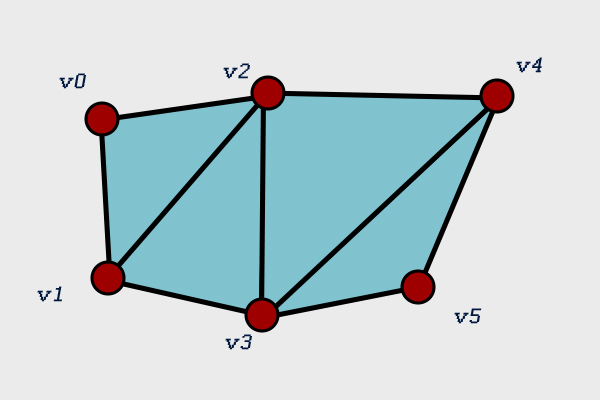
\includegraphics[width=\textwidth]{img/GL_TRIANGLE_STRIP}
%		\\ {\tiny GL\_TRIANGLE\_STRIP}
%	\end{column}
%	\begin{column}{0.3\textwidth}
%		\centering	
%		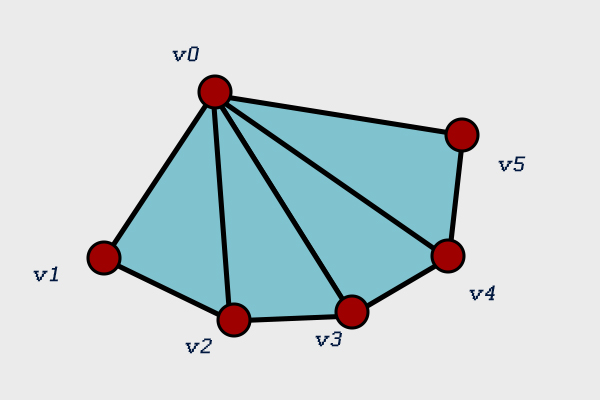
\includegraphics[width=\textwidth]{img/GL_TRIANGLE_FAN}
%		\\ { GL\_TRIANGLE\_FAN}
%	\end{column}
	\begin{column}{0.3\textwidth}
		\centering		
		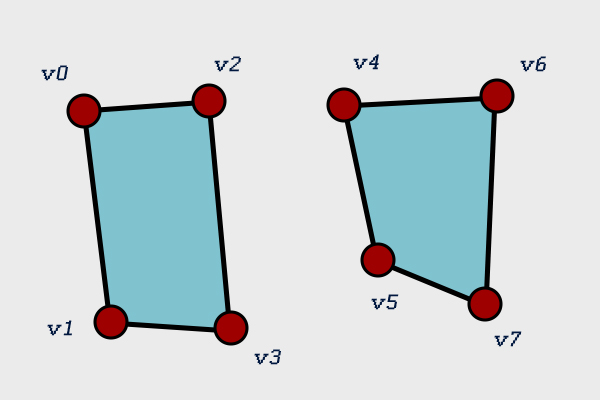
\includegraphics[width=\textwidth]{img/GL_QUADS}
		\\ { GL\_QUADS}
	\end{column}
%	\begin{column}{0.2\textwidth}
%		\centering	
%		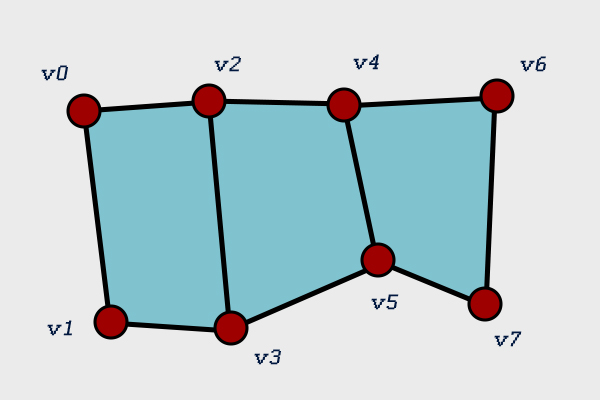
\includegraphics[width=\textwidth]{img/GL_QUAD_STRIP}
%		\\ {\tiny GL\_QUAD\_STRIP}
%	\end{column}
%	\begin{column}{0.2\textwidth}
%		\centering	
%		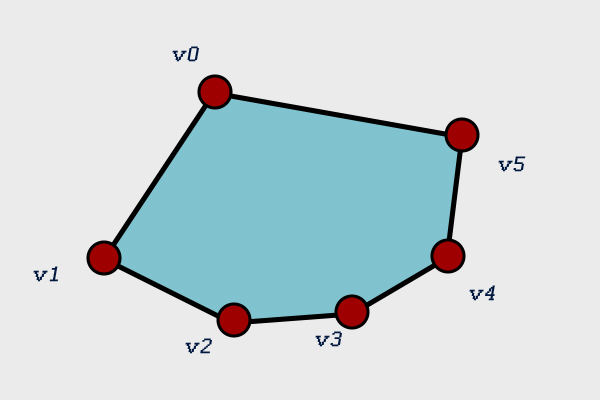
\includegraphics[width=\textwidth]{img/GL_POLYGON}
%		\\ {\tiny GL\_POLYGON}
%	\end{column}
\end{columns}
\end{frame}

\begin{frame}[fragile]
\frametitle{Exemples simples de modélisation : cylindre}
	\vspace{-5mm}
	\begin{columns}[T]
		\begin{column}{0.45\textwidth}
			\begin{block}{Cylindre}
			\centering
				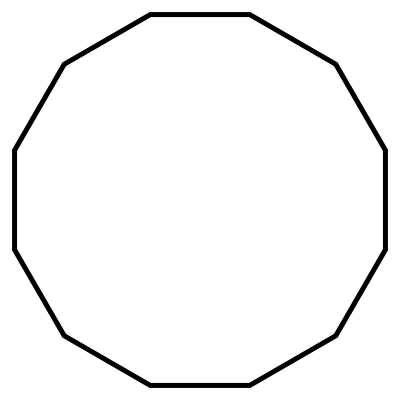
\includegraphics[width=0.6\textwidth]{img/cone_base}
				~\\
				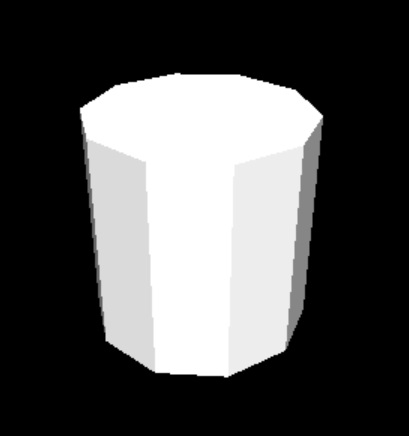
\includegraphics[width=0.6\textwidth]{img/cylindre}
			\end{block}
		\end{column}
		\pause
		\begin{column}{0.45\textwidth}
			\begin{exampleblock}{Réponse}
				\begin{figure}[h]
					\begin{tabular}{c}
						\centering
						\begin{lstlisting}[basicstyle=\small]

for(int i=0; i<p; ++i){
  glBegin(GL_TRIANGLES);
  ... //base inferieure
  glEnd();
  glBegin(GL_TRIANGLES);
  ... //base superieure
  glEnd();
  glBegin(GL_QUADS);
  ... //faces laterales
  glEnd();
}
						\end{lstlisting}
					\end{tabular}
				\end{figure}
			\end{exampleblock}
			\pause
			\begin{exampleblock}{Une autre solution}
				\begin{figure}[h]
					\centering
					\begin{tabular}{c}
						\begin{lstlisting}[basicstyle=\small]
gluCylinder(...);
						\end{lstlisting}
					\end{tabular}
				\end{figure}
			\end{exampleblock}
		\end{column}
	\end{columns}
\end{frame}



\begin{frame}[fragile]
\frametitle{Exemple de modélisation : cône}
	\begin{columns}[T]
		\begin{column}{0.45\textwidth}
			\begin{block}{Cône}
				\centering
				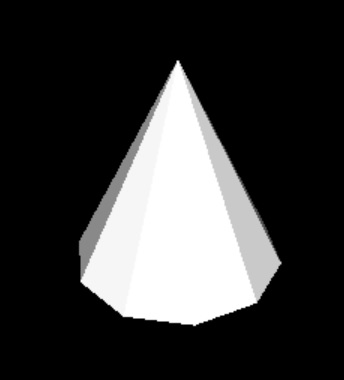
\includegraphics[width=0.75\textwidth]{img/cone}
			\end{block}
		\end{column}
		\pause
		\begin{column}{0.45\textwidth}
			\begin{exampleblock}{Réponse}
				\begin{figure}[h]
					\centering
					\begin{tabular}{c}
						\begin{lstlisting}[basicstyle=\small]

for(int i=0; i<p; ++i){
  glBegin(GL_TRIANGLES);
  ... //face inferieure
  glEnd();
  glBegin(GL_TRIANGLES);
  ... //faces laterales
  glEnd();
}
						\end{lstlisting}
					\end{tabular}
				\end{figure}	
			\end{exampleblock}	
		\end{column}
	\end{columns}
	\pause
	\begin{exampleblock}{Une autre solution}
		\begin{figure}[h]
			\centering
			\begin{tabular}{c}
				\begin{lstlisting}[basicstyle=\small]
glutSolidCone(...);
				\end{lstlisting}
			\end{tabular}
		\end{figure}
	\end{exampleblock}
\end{frame}


\subsection{Commandes avancées}

\begin{frame}{OpenGL est une machine à états}
\begin{block}{Deux nouvelles commandes}
\begin{itemize}
\item glNormal3f
\item glColor3f
\end{itemize}
\end{block}
\begin{block}{Machine à états}
Executer \verb!glColor3f(1,1,1)! choisit la "couleur courante". Tout sera dessiné avec cette couleur jusqu'à ce que la couleur soit changée par une nouvelle exécution de \verb!glColor()!.
\end{block}
\end{frame}

\begin{frame}[fragile]
\frametitle{Commandes à disposition entre \verb!glBegin()! et \verb!glEnd()! (1)}
	\begin{block}{\verb!glVertex3f(x,y,z)!}
	\end{block}
	\begin{block}{\verb!glNormal3f(x,y,z)!}
		Déclarer la normale au polygone que l'on trace.\\
		\alert{Une normale déclarée est utilisée jusqu'à être remplacée}
%		\alert{Utile} : initialiser \verb!glEnable(GL_NORMALIZE);! : normalisation auto.
		\begin{minipage}{\linewidth}
			\begin{columns}[T]
				\begin{column}{0.45\textwidth}
					\begin{exampleblock}{}
						\begin{lstlisting}[basicstyle=\small]
glBegin(GL_QUADS);
  <@\textcolor{red}{glNormal3f(0,1,0);}@>
    glVertex3f(1,0,1);
    glVertex3f(1,0,-1);
    glVertex3f(-1,0,-1);
    glVertex3f(-1,0,1);
glEnd();
						\end{lstlisting}
					\end{exampleblock}
				\end{column}
				\begin{column}{0.45\textwidth}
					\begin{exampleblock}{}
						\begin{lstlisting}[basicstyle=\small]
glBegin(GL_TRIANGLES);
  <@\textcolor{red}{glNormal3f(0,1,0);}@>
    glVertex3f(1,0,1);
    glVertex3f(1,0,-1);
    glVertex3f(-1,0,-1);
  <@\textcolor{red}{glNormal3f(0,1,0);}@>
    glVertex3f(1,0,1);
    glVertex3f(-1,0,-1);
    glVertex3f(-1,0,1);
glEnd();
						\end{lstlisting}
					\end{exampleblock}
				\end{column}
			\end{columns}
		\end{minipage}
	\end{block}
\end{frame}

\begin{frame}[fragile]
\frametitle{Commandes à disposition entre \verb!glBegin()! et \verb!glEnd()! (2)}
	\begin{block}{\verb!glColor3f(r,g,b)!}
		\begin{columns}
			\begin{column}{0.8\textwidth}
				Déclarer la couleur à utiliser dans la suite du programme.\\
				\verb!r!,\verb!g!,\verb!b!,\verb!a! doivent prendre des valeurs entre $0.0$ et $1.0$.\\
				Par défaut : \verb!glColor4d(1,1,1,1);!.\\
				Pour activer la composante alpha : \verb!glEnable(GL_BLEND);!.
			\end{column}
			\begin{column}{0.15\textwidth}
				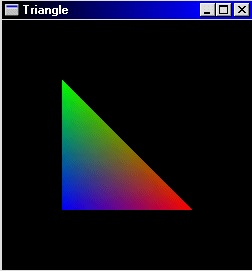
\includegraphics[width=\textwidth]{img/triang}
			\end{column}
		\end{columns}
		\begin{figure}
			\centering
			\begin{tabular}{c}
				\begin{lstlisting}[basicstyle=\small]
glBegin(GL_TRIANGLE);
  glNormal3f(0, 0, 1);
    <@\textcolor{red}{glColor3f(1, 0, 0);}@>
      glVertex3f(,,);
    <@\textcolor{red}{glColor3f(1, 1, 0);}@>
      glVertex3f(,,);
    <@\textcolor{red}{glColor3f(1, 1, 1);}@>
      glVertex3f(,,);
glEnd();
				\end{lstlisting}
			\end{tabular}
		\end{figure}
	\end{block}
\end{frame}

%\begin{frame}[fragile]
%\frametitle{Commandes à disposition entre \verb!glBegin()! et \verb!glEnd()! (3)}
%	\begin{columns}
%		\begin{column}{0.6\textwidth}
%			\begin{block}{\verb!glMaterial?(face, gl\_param, values)!}
%				\verb!face! détermine quelle face est calculée :
%				\begin{itemize}
%					\item \alert{ \verb!GL\_FRONT\_AND\_BACK! }
%				\end{itemize}
%				gl\_param est le paramètre du matériau :
%				\begin{itemize}
%					\item \verb!GL_AMBIENT! : 4 variables $[-1.0,1.0]$
%					\item \verb!GL_DIFFUSE! : 4 variables $[-1.0,1.0]$
%					\item \verb!GL_SPECULAR! : 4 variables $[-1.0,1.0]$
%					\item \verb!GL_EMISSION! : 4 variables $[-1.0,1.0]$
%					\item \verb!GL_SHININESS! : 1 variable $[0,128]$
%				\end{itemize}
%				\verb!values! est un pointeur vers le tableau de paramètres
%			\end{block}
%		\end{column}
%		\begin{column}{0.35\textwidth}
%			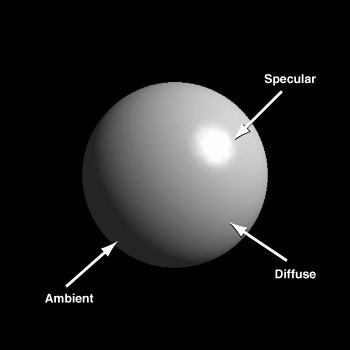
\includegraphics[width=\textwidth]{img/light_material}
%		\end{column}
%	\end{columns}
%\end{frame}

\begin{frame}{Récupération du TP}

\begin{block}{Dans un terminal:}
\begin{itemize}
\item git clone https://github.com/n-stott/mines.git
\end{itemize}
\end{block}

\begin{block}{Architecture}
\begin{itemize}
\item Boids:
\begin{itemize}
\item  le gros TP (plus tard)
\end{itemize}
\item Canvas:
\begin{itemize}
\item exercice de cours (maintenant)
\end{itemize}
\item Supp:
\begin{itemize}
\item supports de cours
\end{itemize}
\end{itemize}
\end{block}

\begin{block}{Compilation}
Dans un terminal, dans le dossier de l'exercice/du TP, exécuter:
\begin{itemize}
\item sh build.sh
\end{itemize}
\end{block}

\end{frame}





\subsection{Transformations géométriques}

\begin{frame}
\frametitle{Les transformations élémentaires}
	\begin{alertblock}{Principe de transformation}
		Chaque commande de transformation transforme le repère de dessin local.
	\end{alertblock}
	\begin{block}{Translation}
		\verb!glTranslatef(x,y,z)! 
	\end{block}
	\begin{block}{Changement d'échelle}
		\verb!glScalef(x,y,z)! multiplie l'échelle par \verb!x!,\verb!y!,\verb!z! dans les directions $x$,$y$,$z$ respectivement.
	\end{block}
	\begin{block}{Rotation autour d'un axe}
		\verb!glRotatef(t,x,y,z)! effectue une rotation de $t$ autour de l'axe $[x\;y\;z]^T$
	\end{block}
\end{frame}

\begin{frame}[fragile]
\frametitle{Modélisation, transformation et animation}
\setbeamercovered{invisible}
	\begin{exampleblock}{Exercice}
		Comment faire pour animer un objet dans une scène ? Par exemple, faire tourner un carré autour d'une de ses diagonales ? Et un cube ?
	\end{exampleblock}
	\pause
	\begin{columns}[T]
		\begin{column}{0.58\textwidth}
			\begin{block}{Solution 1 :}
			%	Animer la position des sommets lors du tracé.
			%	\vspace{-5mm}
				\begin{figure}[h]
				\centering
				\begin{tabular}{c}
				\begin{lstlisting}[basicstyle=\small]
glBegin(GL_QUADS);
  ...
  glVertex3f(cosf(t),sinf(t),0);
  ...
glEnd();
				\end{lstlisting}
				\end{tabular}
				\end{figure}
			\end{block}
		\end{column}
		\begin{column}{0.40\textwidth}
			\begin{block}{Solution 2:}
			%	Tracer un cube et effectuer la transformation nécessaire.
				\begin{figure}[h]
				\centering
				\begin{tabular}{c}
				\begin{lstlisting}[basicstyle=\small]
glRotatef(t,0,0,1);
glBegin(GL_QUADS);
  ...
  glVertex3f(1,0,0);
  ...
glEnd();
glRotatef(-t,0,0,1);
				\end{lstlisting}
				\end{tabular}
				\end{figure}
			\end{block}
		\end{column}
	\end{columns}
	\begin{block}{}
		En général, la 2ème solution est préférable, surtout si les objets sont complexes : calcul sur le GPU et non sur le CPU.
	\end{block}
\end{frame}

\begin{frame}[fragile]
\frametitle{Manipulation de transformations (1)}
	\begin{exampleblock}{Pas très pratique...}
		\begin{columns}
			\begin{column}{0.45\textwidth}
				\begin{block}{}
					Faire toutes les transformations en double, avant et après avoir tracé mon objet ?
				\end{block}
			\end{column}
			\begin{column}{0.45\textwidth}
				\begin{block}{}
					\begin{figure}[h]
						\centering
						\begin{tabular}{c}
							\begin{lstlisting}
glRotatef(t,0,0,1);
...
glRotatef(-t,0,0,1);
							\end{lstlisting}
						\end{tabular}
					\end{figure}
				\end{block}
			\end{column}
		\end{columns}
	\end{exampleblock}
	\pause
	\begin{block}{Pile de matrices : sauvegarder un état de transformation}
		On choisit la pile de matrices sur laquelle on agit avec \verb!glMatrixMode( GL_MODELVIEW | GL_PROJECTION )!.
		\begin{itemize}
			\item \verb!glLoadIdentity()! : annuler toutes les transformations
			\item \verb!glPushMatrix()! : sauvegarder l'état de transformation courant
			\item \verb!glPopMatrix()! : retour à l'état précédemment enregistré
		\end{itemize}
	\end{block}
\end{frame}

\begin{frame}[fragile]
\frametitle{Manipulation de transformations (2)}
\begin{exampleblock}{Beaucoup plus pratique}
On reprend l'exemple précédent :
\begin{columns}
	\begin{column}{0.45\textwidth}
		\begin{block}{}
			\begin{figure}[h]
			\centering
			\begin{tabular}{c}
			\begin{lstlisting}
glRotatef(t,0,0,1);
glTranslatef(4,3,1);
...
glTranslatef(-4,-3,-1);
glRotatef(-t,0,0,1);
			\end{lstlisting}
			\end{tabular}
			\end{figure}
		\end{block}
	\end{column}
	\begin{column}{0.45\textwidth}
		\begin{block}{}
			\begin{figure}[h]
			\centering
			\begin{tabular}{c}
			\begin{lstlisting}
glPushMatrix();
  glRotatef(t,0,0,1);
  glTranslatef(4,3,1);
  ...
glPopMatrix();
			\end{lstlisting}
			\end{tabular}
			\end{figure}
		\end{block}
	\end{column}
\end{columns}
\end{exampleblock}
\end{frame}

%\subsection{L'éclairage}
%
%\begin{frame}[fragile]
%\frametitle{L'éclairage dans OpenGL}
%\begin{columns}
%\begin{column}{0.5\textwidth}
%\begin{block}{Type d'ombrage :}
%La commande  \verb!glShadeModel(??)! permet de choisir entre 2 types d'ombrages :
%\begin{itemize}
%	\item \verb!GL_FLAT!
%	\item \verb!GL_SMOOTH!
%\end{itemize}
%\centering
%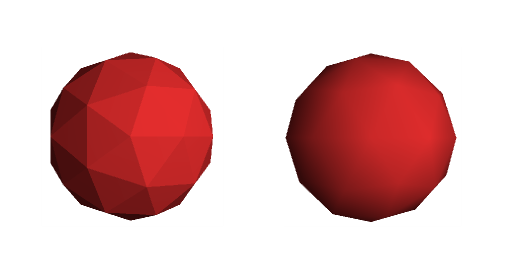
\includegraphics[width=0.8\textwidth]{img/shademodel}
%\end{block}
%\end{column}
%%\begin{column}{0.45\textwidth}
%%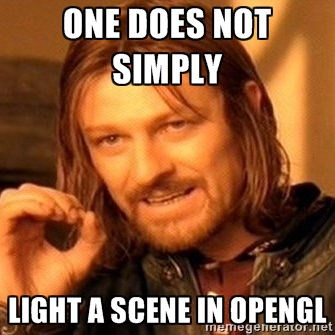
\includegraphics[width=\textwidth]{img/onedoesnotsimply}
%%\end{column}
%\end{columns}
%\end{frame}
%
%\begin{frame}
%\frametitle{Le modèle d'éclairage dans OpenGL}
%
%\begin{columns}
%\begin{column}{0.45\textwidth}
%\begin{block}{Composantes lumineuses}
%\begin{itemize}
%	\item Composante \'Emissive
%	\item Composante Ambiante
%	\item Composante Diffuse
%	\item Composante Spéculaire
%\end{itemize}
%\end{block}
%\end{column}
%\begin{column}{0.45\textwidth}
%\begin{block}{Types de sources lumineuses}
%\begin{itemize}
%	\item Source Ambiante
%	\item Source Ponctuelle
%	\item Source Directionnelle
%	\item Source Spot
%\end{itemize}
%\end{block}
%\end{column}
%\end{columns}
%~\\
%~\\
%\begin{columns}
%\begin{column}{0.45\textwidth}
%	\centering
%	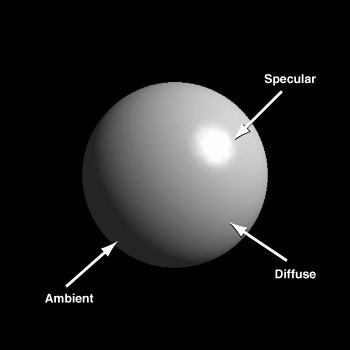
\includegraphics[width=0.7\textwidth]{img/light_material}
%\end{column}
%\begin{column}{0.45\textwidth}
%	\centering
%	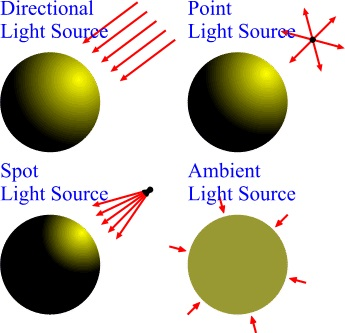
\includegraphics[width=0.7\textwidth]{img/lighttypes}
%\end{column}
%\end{columns}
%\end{frame}
%
%\begin{frame}[fragile]
%\frametitle{Utiliser les lumières}
%\begin{block}{Les lumières dans OpenGL}
%\begin{itemize}
%	\item OpenGL sait gérer jusqu'à 8 sources de lumières simultanément,
%	\item Elles sont nommées \verb!GL_LIGHT!$i$, avec $0 \leq i < 8$.
%\end{itemize}
%\end{block}
%\begin{block}{Activation}
%\begin{itemize}
%	\item{ Configuration d'OpenGL pour utiliser les lumières :
%	\begin{center}
%		\verb!glEnable(GL_LIGHTING);!\\
%	\end{center}
%	}
%	\item{ Activation d'une lumière :
%	\begin{center}
%		\verb!glEnable(GL_LIGHT0);!
%	\end{center}
%	}
%	\item{ On déclare les couleurs de faces comme des matériaux :
%		\verb!glEnable(GL_COLOR_MATERIAL);!
%	}
%\end{itemize}
%\end{block}
%\end{frame}
%
%\begin{frame}[fragile]
%\frametitle{Les commandes de lumière}
%\begin{block}{\verb!glLight(gl\_light,gl\_param,values)!}
%Les paramètres ajustables et leurs valeurs :
%\begin{itemize}
%	\item \verb!GL_AMBIENT! : 4 variables (intensité RGBA)
%	\item \verb!GL_DIFFUSE! : 4 variables (intensité RGBA)
%	\item \verb!GL_SPECULAR! : 4 variables (intensité RGBA)
%	\item \verb!GL_POSITION! : 4 variables (position XYZW)
%	\item \verb!GL_SPOT_DIRECTION! : 3 variables (vecteur direction)
%\end{itemize}
%\end{block}
%\begin{block}{\verb!glLightModel(gl\_param,gl\_value)! (Description)}
%Offrir plus de contrôle sur la compréhension des paramètres lumineux :
%\begin{itemize}
%	\item \verb!GL_LIGHT_MODEL_AMBIENT! : contrôle l'intensité de la lumière ambiante
%	\item \verb!GL_LIGHT_MODEL_COLOR_CONTROL! : contrôle des éventuels conflits entre textures et lumière
%\end{itemize}
%\end{block}
%\end{frame}

\subsection{Gestion de la caméra}

\begin{frame}
\frametitle{Utilisation simple de la caméra}
\begin{block}{Une fonction GLU utile}
	\begin{itemize}
		\item{\verb!gluLookAt(eyeX,eyeY,eyeZ,atX,atY,atZ,upX,upY,upZ)!
%			\begin{itemize}
%				\item \verb!fovy! : ouverture verticale en degrés
%				\item \verb!aspect! : ratio largeur/hauteur de l'image
%				\item \verb!zNear! : plan de coupure proche
%				\item \verb!zFar! : plan de couûre lointain
%			\end{itemize}
		}
	\end{itemize}
	\centering
	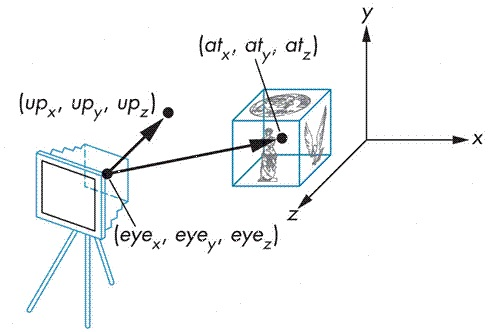
\includegraphics[width=0.5\textwidth]{img/ortho}\\
	On manipule des matrices géométriques :\\
	\verb!glMatrixMode(GL\_MODELVIEW);!
\end{block}
\end{frame}


\section{Les fonctions principales GLUT}

%\begin{frame}{}
%
%\begin{center}
%Présentation du TP
%\end{center}
%
%\end{frame}

%\begin{frame}[fragile]
%\frametitle{La fonction Main}
%\begin{block}{Contenu}
%La fonction main doit :
%\begin{itemize}
%	\item initialiser GLUT : \verb!glutInit(&argc,argv);!
%	\item paramétrer l'affichage avec \verb!glutInitDisplayMode( ... );! :\\ \verb!GLUT_RGBA!, \verb!GLUT_DEPTH!, \verb!GLUT_SINGLE! ou \verb!GLUT_DOUBLE!
%	\item créer la fenêtre : \verb!glutCreateWindow("C'est bientôt fini ;)");!
%	\item initialiser les variables/objets du programme
%	\item {déclarer les fonctions
%		\begin{itemize}
%			\item de dessin : \verb!glutDisplayFunc( ... );!
%			\item de redimensionnement : \verb!glutReshapeFunc( ... );!
%			\item d'interaction souris : \verb!glutMouseFunc( ... );!
%			\item d'interaction clavier : \verb!glutKeyboardFunc( ... );!
%			\item d'évolution autonome : \verb!glutIdleFunc( ... );!
%			\item de temporisation : \verb!glutTimerFunc( ... );!
%		\end{itemize}
%	}
%	\item lancer la boucle infinie : \verb!glutMainLoop();!
%\end{itemize}
%\end{block}
%\end{frame}
%
%\begin{frame}{Autres fonctions (1)}
%\begin{block}{Fonction de dessin}
%Donnée en paramètre de \verb!glutDisplayFunc(...)!\\
%Elle ne prend rien en paramètre.\\
%Son rôle est de tracer l'image courante :
%\begin{itemize}
%	\item effacer l'image précédente : \verb!glClear(GL\_COLOR\_BUFFER\_BIT);!
%	\item dessiner ce que l'utilisateur souhaite
%	\item demander de l'afficher : \verb!glFlush();! ou \verb!glSwapBuffers();!
%\end{itemize}
%\end{block}
%\pause
%\begin{block}{Fonction de redimensionnement}
%Donnée en paramètre de \verb!glutReshapeFunc( ... );!\\
%Elle prend en paramètre les dimensions du viewport.\\
%Elle doit assurer la cohérence de la fenêtre de tracé :
%\begin{itemize}
%	\item déclarer le viewport : \verb!glViewport(x1,y1,x2,y2);!
%	\item charger les paramètres caméra initiaux
%\end{itemize}
%\end{block}
%\end{frame}
%
%\begin{frame}{Autres fonctions (2)}
%\begin{block}{Fonction d'interaction souris}
%Donnée en paramètre de \verb!glutMouseFunc( ... );!\\
%Elle prend en paramètre le bouton activé, l'état du bouton et la position écran lors de l'action.
%\begin{itemize}
%	\item Le bouton prend les valeurs \verb!GLUT\_LEFT/MIDDLE/RIGHT\_BUTTON!
%	\item L'état prend les valeurs \verb!GLUT\_UP! et \verb!GLUT\_DOWN!
%\end{itemize}
%\end{block}
%\pause
%\begin{block}{Fonction d'interaction clavier}
%Donnée en paramètre de \verb!glutKeyboardFunc( ... );!\\
%Elle prend en paramètre la touche activée et la position écran de la souris lors de l'action.
%\end{block}
%\end{frame}
%
%\begin{frame}{Autres fonctions (3)}
%\begin{block}{Fonction d'évolution autonome}
%Donnée en paramètre de \verb!glutIdleFunc( ... );!\\
%Appelée lorsqu'aucune action n'est déclenchée, elle ne prend aucun paramètre. C'est la fonction qui calcule le nouvel état du système, etc.
%\end{block}
%\pause
%\begin{block}{Fonction de temporisation}
%Donnée en paramètre de \verb!glutTimerFunc( ... );!\\
%Fonction avancée qui permet d'introduire des paramètres temporels dans le programme.\\
%\verb!glutTimerFunc(DeltaT,timer,0)! appelle la fonction de temporisation \verb!timer! au moins toutes les \verb!DeltaT! ms.
%\end{block}
%\pause
%\begin{block}{Fonction d'actualisation}
%\verb!glutPostRedisplay();! est la fonction qui demande à GLUT de calculer et d'afficher une nouvelle image sur l'écran.
%\end{block}
%\end{frame}


\begin{frame}
\frametitle{}
\begin{center}
{\Huge TP: ~\\
~\\
Simulation d'une flotte de robots
}
\end{center}
%\begin{figure}[h]
%\centering
%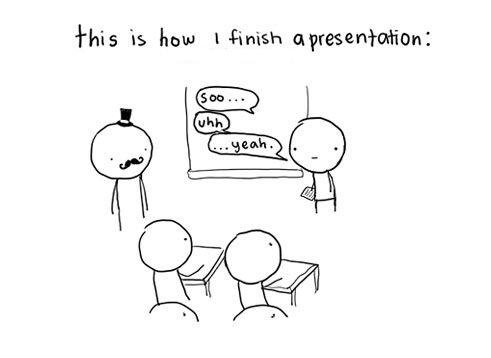
\includegraphics[width=0.8\textwidth]{img/end}
%\end{figure}
\end{frame}

\section{La librairie mathématique Eigen}

\begin{frame}
\frametitle{Commandes principales}
\begin{block}{Eigen::Vector3f v}
\begin{itemize}
\item Vecteur de $3$ floats x,y,z: Eigen::Vector3f(x,y,z)
\item Acces aux valeurs: v[i]
\item Compatible avec les opérations standards sur des vecteur: 3*u - 2*v est une syntaxe valide
\end{itemize}
\end{block}


\begin{block}{Produit scalaire $\langle u , v \rangle$}
\begin{itemize}
\item Calculé par u.dot(v)
\item Norme d'un vecteur: sqrt(u.dot(u)) ou u.norm()
\item Vecteur normalisé: $\textrm{u}_{\textrm{norm}}$ = u.normalized()
\item Autre version (inplace): u.normalize()
\end{itemize}
\end{block}

\begin{block}{Produit vectoriel $u \wedge v$}
\begin{itemize}
\item Calculé par u.cross(v)
\end{itemize}
\end{block}

\end{frame}


%\fi

\end{document}